\documentclass[12pt]{article}
\linespread{1.2}
\usepackage[margin=2cm]{geometry}
\usepackage[utf8]{inputenc}
\usepackage{amsfonts}
\usepackage{amsmath}
\usepackage{multicol}
\usepackage{amsthm}
\usepackage{amssymb,scrextend}
\usepackage{graphicx,tikz}
\newtheorem{dfn}{Definition}
\renewcommand{\qed}{\hfill$\blacksquare$}
\let\newproof\proof
\renewenvironment{proof}{\vspace{1em}\begin{addmargin}[2em]{0em}\begin{newproof}}{\end{newproof}\end{addmargin}\qed}
\newenvironment{theorem}[2][Theorem]{\begin{trivlist}
\item[\hskip \labelsep {\bfseries #1} \hskip \labelsep {\bfseries #2.}]}{\end{trivlist}}
\newenvironment{example}[2][Example]{\begin{trivlist}
\item[\hskip \labelsep {\bfseries #1} \hskip \labelsep {\bfseries #2.}]}{\end{trivlist}}
\newenvironment{lemma}[2][Lemma]{\begin{trivlist}
\item[\hskip \labelsep {\bfseries #1} \hskip \labelsep {\bfseries #2.}]}{\end{trivlist}}
\newenvironment{exercise}[2][Exercise]{\begin{trivlist}
\item[\hskip \labelsep {\bfseries #1} \hskip \labelsep {\bfseries #2.}]}{\end{trivlist}}
\newenvironment{problem}[2][Problem]{\begin{trivlist}
\item[\hskip \labelsep {\bfseries #1} \hskip \labelsep {\bfseries #2.}]}{\end{trivlist}}
\newenvironment{corollary}[2][Corollary]{\begin{trivlist}
\item[\hskip \labelsep {\bfseries #1} \hskip \labelsep {\bfseries #2.}]}{\end{trivlist}}
\usepackage{fancyhdr,enumitem,changepage,url}
\pagestyle{fancy}
\author{Warren Atkison}
\date{\today}
\setlength{\headheight}{15pt}
\begin{document}
\fancyhf{}
\fancyhead[L]{Warren Atkison}
\fancyhead[C]{Experiment 14.9}
\fancyhead[R]{\today}
\fancyfoot[R]{\thepage}

\subsection*{Goal}
In this experiment you are asked to identify the iterated function systems that produced certain fractals as their attractors.

\subsection*{Procedure}
In Figures 14.20 and 14.21 we have displayed six different fractals, each contained in the unit square in the plane. First determine how many self-similar pieces you see in each set, and then figure out the contraction factor. Then write down explicitly the formulas in the iterated function system that generated these images. And, finally, determine the fractal dimension of each set.
\begin{itemize}
	\item[(a)] There appears to be 5 self similar pieces, with a contraction factor of 3. The itereative formula that generates this image is as follows:
	\begin{align*}
		f_1(\vec{x}) &= \frac{1}{3} \begin{bmatrix}
			x \\
			y
		\end{bmatrix} + \begin{bmatrix}
			0 \\
			2/3
		\end{bmatrix} \\
		f_2(\vec{x}) &= \frac{1}{3} \begin{bmatrix}
			x \\
			y
		\end{bmatrix} + \begin{bmatrix}
			1/3 \\
			2/3
		\end{bmatrix} \\
		f_3(\vec{x}) &= \frac{1}{3} \begin{bmatrix}
			x \\
			y
		\end{bmatrix} + \begin{bmatrix}
			2/3 \\
			2/3
		\end{bmatrix} \\
		f_4(\vec{x}) &= \frac{1}{3} \begin{bmatrix}
			x \\
			y
		\end{bmatrix} + \begin{bmatrix}
			1/3 \\
			1/3
		\end{bmatrix} \\
		f_5(\vec{x}) &= \frac{1}{3} \begin{bmatrix}
			x \\
			y
		\end{bmatrix} + \begin{bmatrix}
			1/3 \\
			0
		\end{bmatrix}
	\end{align*}
	The dimension of our fractal is
	\[
		D = \frac{\log 5}{\log 3} \approx 1.465
	\]
	\item[(b)] There appears to be 6 self similar pieces, with a contraction factor of 3. The iterative formula that generates this image is as follows:
	\begin{align*}
		f_1(\vec{x}) &= \frac{1}{3} \begin{bmatrix}
			x \\
			y
		\end{bmatrix} + \begin{bmatrix}
			1/6 \\
			2/3
		\end{bmatrix} \\
		f_2(\vec{z}) &= \frac{1}{3} \begin{bmatrix}
			x \\
			y
		\end{bmatrix} + \begin{bmatrix}
			1/2 \\
			2/3
		\end{bmatrix} \\
		f_3(\vec{x}) &= \frac{1}{3} \begin{bmatrix}
			x \\
			y
		\end{bmatrix} + \begin{bmatrix}
			0 \\
			1/3
		\end{bmatrix} \\
		f_4(\vec{x}) &= \frac{1}{3}\begin{bmatrix}
			x \\
			y
		\end{bmatrix} + \begin{bmatrix}
			2/3 \\
			1/3
		\end{bmatrix} \\
		f_5(\vec{x}) &= \frac{1}{3}\begin{bmatrix}
			x \\
			y
		\end{bmatrix} + \begin{bmatrix}
			1/6 \\
			0
		\end{bmatrix} \\
		f_6(\vec{x}) &= \frac{1}{3}\begin{bmatrix}
			x \\
			y
		\end{bmatrix} + \begin{bmatrix}
			1/2 \\
			0
		\end{bmatrix}
	\end{align*}
	The dimension of our fractal is
	\[
		D = \frac{\log 6}{\log 3} \approx 1.631
	\]
	\item[(c)] There appears to be 5 self similar pieces, with a contraction factor of 3. The itereative formula that generates this image is as follows:
	\begin{align*}
		f_1(\vec{x}) &= \frac{1}{3} \begin{bmatrix}
			x \\
			y
		\end{bmatrix} + \begin{bmatrix}
			0 \\
			2/3
		\end{bmatrix} \\
		f_2(\vec{x}) &= \frac{1}{3} \begin{bmatrix}
			x \\
			y
		\end{bmatrix} + \begin{bmatrix}
			1/3 \\
			2/3
		\end{bmatrix} \\
		f_3(\vec{x}) &= \frac{1}{3} \begin{bmatrix}
			x \\
			y
		\end{bmatrix} + \begin{bmatrix}
			0 \\
			1/3
		\end{bmatrix} \\
		f_4(\vec{x}) &= \frac{1}{3} \begin{bmatrix}
			x \\
			y
		\end{bmatrix} + \begin{bmatrix}
			1/3 \\
			1/3
		\end{bmatrix} \\
		f_5(\vec{x}) &= \frac{1}{3} \begin{bmatrix}
			x \\
			y
		\end{bmatrix} + \begin{bmatrix}
			2/3 \\
			0
		\end{bmatrix}
	\end{align*}
	The dimension of our fractal is
	\[
		D = \frac{\log 5}{\log 3} \approx 1.465
	\]
	\item[(d)] There appears to be 4 self similar pieces, with a contraction factor of 2. The itereative formula that generates this image is as follows:
	\begin{align*}
		f_1(\vec{x}) &= 2 \begin{bmatrix}
			x \\
			y
		\end{bmatrix} + \begin{bmatrix}
			1/4 \\
			1/2
		\end{bmatrix} \\
		f_2(\vec{x}) &= 2 \begin{bmatrix}
			x \\
			y
		\end{bmatrix} + \begin{bmatrix}
			0 \\
			1/4
		\end{bmatrix} \\
		f_3(\vec{x}) &= 2 \begin{bmatrix}
			x \\
			y
		\end{bmatrix} + \begin{bmatrix}
			1/2 \\
			1/4
		\end{bmatrix} \\
		f_4(\vec{x}) &= 2 \begin{bmatrix}
			x \\
			y
		\end{bmatrix} + \begin{bmatrix}
			1/4 \\
			0
		\end{bmatrix} 
	\end{align*}
	The dimension of our fractal is
	\[
		D = \frac{\log 4}{\log 2} = 2
	\]
	\item[(e)] There appears to be 5 self similar pieces, with a contraction factor of 3. The itereative formula that generates this image is as follows:
	\begin{align*}
		f_1(\vec{x}) &= \frac{1}{3} \begin{bmatrix}
			x \\
			y
		\end{bmatrix} + \begin{bmatrix}
			0 \\
			2/3
		\end{bmatrix} \\
		f_2(\vec{x}) &= \frac{1}{3} \begin{bmatrix}
			x \\
			y
		\end{bmatrix} + \begin{bmatrix}
			1/3 \\
			2/3
		\end{bmatrix} \\
		f_3(\vec{x}) &= \frac{1}{3} \begin{bmatrix}
			x \\
			y
		\end{bmatrix} + \begin{bmatrix}
			0 \\
			1/3
		\end{bmatrix} \\
		f_4(\vec{x}) &= \frac{1}{3} \begin{bmatrix}
			x \\
			y
		\end{bmatrix} + \begin{bmatrix}
			2/3 \\
			1/3
		\end{bmatrix} \\
		f_5(\vec{x}) &= \frac{1}{3} \begin{bmatrix}
			x \\
			y
		\end{bmatrix} + \begin{bmatrix}
			2/3 \\
			0
		\end{bmatrix}
	\end{align*}
	The dimension of our fractal is
	\[
		D = \frac{\log 5}{\log 3} \approx 1.465
	\]
	\item[(f)] There appears to be 5 self similar pieces, with a contraction factor of 3. The itereative formula that generates this image is as follows:
	\begin{align*}
		f_1(\vec{x}) &= \frac{1}{3} \begin{bmatrix}
			x \\
			y
		\end{bmatrix} + \begin{bmatrix}
			1/3 \\
			2/3
		\end{bmatrix} \\
		f_2(\vec{x}) &= \frac{1}{3} \begin{bmatrix}
			x \\
			y
		\end{bmatrix} + \begin{bmatrix}
			0 \\
			1/3
		\end{bmatrix} \\
		f_3(\vec{x}) &= \frac{1}{3} \begin{bmatrix}
			x \\
			y
		\end{bmatrix} + \begin{bmatrix}
			1/3 \\
			1/3
		\end{bmatrix} \\
		f_4(\vec{x}) &= \frac{1}{3} \begin{bmatrix}
			x \\
			y
		\end{bmatrix} + \begin{bmatrix}
			2/3 \\
			1/3
		\end{bmatrix} \\
		f_5(\vec{x}) &= \frac{1}{3} \begin{bmatrix}
			x \\
			y
		\end{bmatrix} + \begin{bmatrix}
			1/3 \\
			0
		\end{bmatrix}
	\end{align*}
	The dimension of our fractal is
	\[
		D = \frac{\log 5}{\log 3} \approx 1.465
	\]

\end{itemize}
\subsection*{Results}
In a brief essay, explain why you were led to choose the iterated function system that produced one of these images. Explain with pictures what each linear contraction in your system does to the unit square in the plane.
\paragraph{}
Let's take image (b). The iterated function system was created to have a cotraction factor of 3, and map our pre-image to 6 different places on the unit square. In this case, we are mapping a hexagon to six different smaller hexagons, a third of the size of the original, and we are mapping (0,0) to (1/6,2/3), (1/2,2/3), (0,1/3), (2/3,1/3), (1/6,0), and (1/2,0). Here is the first and second iteration of our IFS on the unit square.
\begin{center}

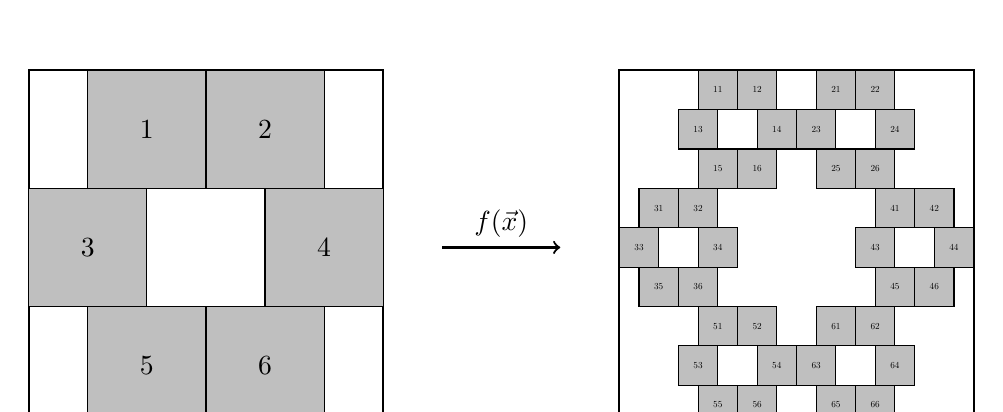
\begin{tikzpicture}[scale=1.5]
  \draw[thick] (0,0) rectangle (3,3);
  
  \foreach \x in {1/2,1.5} {
    \foreach \y in {0,2} {
      \filldraw[fill=gray!50, draw=black] (\x,\y) rectangle (\x+1,\y+1);
    }
  }
  \foreach \x in {0,2} {
    \foreach \y in {1} {
      \filldraw[fill=gray!50, draw=black] (\x,\y) rectangle (\x+1,\y+1);
    }
  }
  \draw[->, thick] (3.5,1.5) -- (4.5,1.5) node[midway, above] {$f(\vec{x})$};
  \draw[thick] (5,0) rectangle (8,3);

	  %\draw[thick] (\x,\y) rectangle (\x+1,\y+1);
  
  	  \foreach \x in {5+1/2+1/6,6,6+1/2+1/6,7} {
    	    \foreach \y in {0,2/3,2,2+2/3} {
      	      \filldraw[fill=gray!50, draw=black] (\x,\y) rectangle (\x+1/3,\y+1/3);
    	  }
  	}	
  	  \foreach \x in {5+1/2,5+2/3+1/2,7-1/2,7+2/3-1/2} {
     	    \foreach \y in {1/3,2+1/3} {
      	      \filldraw[fill=gray!50, draw=black] (\x,\y) rectangle (\x+1/3,\y+1/3);
    	  }
  	}

	%\draw[thick] (\x,\y) rectangle (\x+1,\y+1);

  	  \foreach \x in {5+1/6,6-1/2,7+1/6,7+1/2} {
    	    \foreach \y in {1,1+2/3} {
      	      \filldraw[fill=gray!50, draw=black] (\x,\y) rectangle (\x+1/3,\y+1/3);
    	  }
  	}	
  	  \foreach \x in {5,5+2/3,7,7+2/3} {
     	    \foreach \y in {1+1/3} {
      	      \filldraw[fill=gray!50, draw=black] (\x,\y) rectangle (\x+1/3,\y+1/3);
    	  }
  	}

	\node at (1,2.5) {1};
	\node at (2,2.5) {2};
	\node at (0.5,1.5) {3};
	\node at (2.5,1.5) {4};
	\node at (1,0.5) {5};
	\node at (2,0.5) {6};

	\foreach \x in {5+1/2+1/3} {
		\foreach \y in {2+5/6} {
			\node[scale=0.333] at (\x,\y) {11};
			\node[scale=0.333] at (\x+1/3,\y) {12};
			\node[scale=0.333] at (\x-1/6,\y-1/3) {13};
			\node[scale=0.333] at (\x+1/2,\y-1/3) {14};
			\node[scale=0.333] at (\x,\y-2/3) {15};
			\node[scale=0.333] at (\x+1/3,\y-2/3) {16};
		}
	}

	\foreach \x in {7-1/6} {
		\foreach \y in {2+5/6} {
			\node[scale=0.333] at (\x,\y) {21};
			\node[scale=0.333] at (\x+1/3,\y) {22};
			\node[scale=0.333] at (\x-1/6,\y-1/3) {23};
			\node[scale=0.333] at (\x+1/2,\y-1/3) {24};
			\node[scale=0.333] at (\x,\y-2/3) {25};
			\node[scale=0.333] at (\x+1/3,\y-2/3) {26};
		}
	}

	\foreach \x in {5+1/2+1/3} {
		\foreach \y in {5/6} {
			\node[scale=0.333] at (\x,\y) {51};
			\node[scale=0.333] at (\x+1/3,\y) {52};
			\node[scale=0.333] at (\x-1/6,\y-1/3) {53};
			\node[scale=0.333] at (\x+1/2,\y-1/3) {54};
			\node[scale=0.333] at (\x,\y-2/3) {55};
			\node[scale=0.333] at (\x+1/3,\y-2/3) {56};
		}
	}

	\foreach \x in {7-1/6} {
		\foreach \y in {5/6} {
			\node[scale=0.333] at (\x,\y) {61};
			\node[scale=0.333] at (\x+1/3,\y) {62};
			\node[scale=0.333] at (\x-1/6,\y-1/3) {63};
			\node[scale=0.333] at (\x+1/2,\y-1/3) {64};
			\node[scale=0.333] at (\x,\y-2/3) {65};
			\node[scale=0.333] at (\x+1/3,\y-2/3) {66};
		}
	}

	\foreach \x in {5+1/3} {
		\foreach \y in {1+5/6} {
			\node[scale=0.333] at (\x,\y) {31};
			\node[scale=0.333] at (\x+1/3,\y) {32};
			\node[scale=0.333] at (\x-1/6,\y-1/3) {33};
			\node[scale=0.333] at (\x+1/2,\y-1/3) {34};
			\node[scale=0.333] at (\x,\y-2/3) {35};
			\node[scale=0.333] at (\x+1/3,\y-2/3) {36};
		}
	}

	\foreach \x in {8-2/3} {
		\foreach \y in {1+5/6} {
			\node[scale=0.333] at (\x,\y) {41};
			\node[scale=0.333] at (\x+1/3,\y) {42};
			\node[scale=0.333] at (\x-1/6,\y-1/3) {43};
			\node[scale=0.333] at (\x+1/2,\y-1/3) {44};
			\node[scale=0.333] at (\x,\y-2/3) {45};
			\node[scale=0.333] at (\x+1/3,\y-2/3) {46};
		}
	}

\end{tikzpicture}

\end{center}
Where $f_1(\vec{x}) \to 1$, $f_2(\vec{x}) \to 2$, and etc.
\end{document}
